% Origen: Secciones/PI - Conceptos de diseno en HW.md
% (antes "PI - Introducción al diseno en HW"; los labels conservan el prefijo
% intro-hw). El archivo se llama cap5 por orden de creación.
\chapter{Conceptos de diseño de hardware}
\label{C:intro-hw}

% Figuras de ESTE capítulo + las compartidas. Siempre al principio del archivo.
\graphicspath{{figs/cap5/}{figs/comunes/}}

\begin{destacado}
En este capítulo se describen todos los detalles que nos hubiera gustado saber
para comenzar el desarrollo de herramientas que utilicen módulos de hardware
programable: desde las capacidades del mismo, cómo comunicarlo y cuáles son las
abstracciones, hasta cómo se verifica el funcionamiento correcto en cada una de
las etapas.
\end{destacado}

%==============================================================================
\section{Diseño digital}
\label{S:intro-hw-diseno-digital}

En este capítulo se introducen las técnicas y conceptos esenciales para el
diseño y la verificación de HW. Comenzamos explicando los elementos de diseño;
los pasos primordiales son los siguientes:
\begin{enumerate}
  \item Plantear el sistema a implementar o la posible mejora.
  \item Simular la situación con Monte-Carlo.
  \item Analizar las ventanas obtenidas y los recursos empleados.
  \item Implementar en HW.
  \item Implementar el SW de adquisición.
\end{enumerate}
A continuación describimos los detalles de la parte de la implementación en HW.

%==============================================================================
\section{Elementos de diseño}
\label{S:intro-hw-elementos}

\subsection{\emph{Waveforms}}
\label{S:intro-hw-waveforms}

Son representaciones temporales de las señales. Lo más importante a la hora de
leerlas es:
\begin{enumerate}
  \item Identificar los \emph{clocks} y los dominios de reloj en juego.
  \item Simplificar mentalmente el sistema: muchas señales indican el comienzo o
    el fin de una transacción, de modo que determinan las ``vallas''.
  \item Prestar atención a las \textbf{flechas}: indican qué señal depende de
    cuál (por ejemplo, un \codigo{ack} que sólo puede subir después del pedido)
    y son extremadamente útiles para analizar el flujo del procedimiento. La
    especificación de AXI usa la misma convención para las dependencias entre
    las señales del \emph{handshake}~\citecap{AMBAAXI}{A3}.
\end{enumerate}

\subsection{Mecanismos de transferencia de datos}
\label{S:intro-hw-transferencia}

Se refiere a cómo \textbf{interpretar y estructurar la comunicación}: quién
inicia cada transferencia, quién confirma que llegó y quién puede frenar a
quién. Podemos identificar tres esquemas de comunicación, que se presentan en la
Fig.~\ref{f:intro-hw-tipos-control}.

\begin{figure}[H]
\centering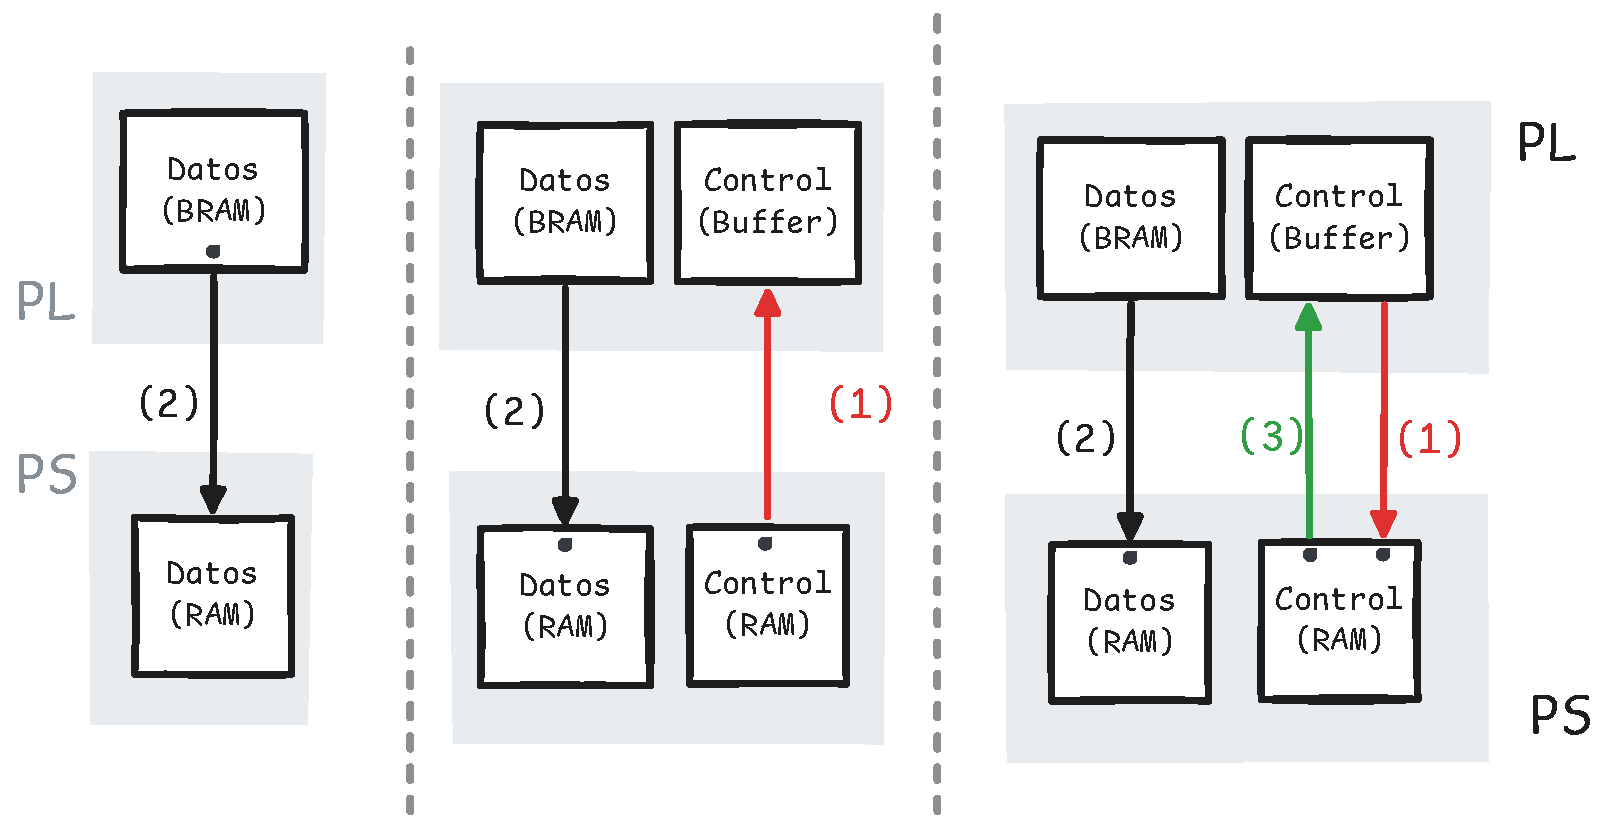
\includegraphics{cap5_tipos_control_flujo}
\caption[Esquemas de transferencia de datos entre PL y PS]{%
Esquemas de transferencia de datos entre PL y PS. (a) \emph{Fire and forget},
\emph{master}: PL. Se tiene un flujo posiblemente constante de datos. (b) Sin
\emph{feedback}, \emph{master}: PS. Esquema intermedio con validez limitada. (c) \emph{Handshake}
completo, \emph{master}: PS. \emph{Handshake} de comunicación completo; en este caso
implementado para \emph{slave} bloqueante (una única transacción en vuelo).
\label{f:intro-hw-tipos-control}}
\end{figure}

Para la comunicación de la Fig.~\ref{f:intro-hw-tipos-control}(a), del tipo
\textbf{\emph{stream}} llamada \emph{fire and forget}, se fijan las condiciones como
especificación del iniciador de trama, y el terminador puede estar especificado
o estar implícito por diseño. El receptor no tiene forma de frenar al emisor:
AXI4-Stream, por ejemplo, permite omitir la señal de vuelta \codigo{TREADY}, que
entonces se considera siempre en alto~\cite{AXIStream}.

Generalmente estas comunicaciones se realizan por el mismo \textbf{canal
físico}; la separación entre los distintos canales es lógica, porque cada uno
tiene una dirección física fija y distinta.

Es importante ver que las flechas indican el sentido de la transferencia de
datos, mientras que el punto indica quién arranca la transferencia: la
diferencia está en si se emite una \emph{request} o una \emph{response}. Por
ejemplo, en el esquema \emph{fire and forget} el \emph{master} es la PL, mientras que
en los esquemas sin \emph{feedback} y de \emph{handshake} completo el \emph{master} es el PS. Siempre
vamos a encontrar que una interfaz tiene un rol (\emph{master}/\emph{slave}) asociado, porque
es una abstracción útil: un canal bidireccional siempre puede interpretarse como
dos canales unidireccionales. Esto es extremadamente útil cuando hay una
asimetría en los roles, por ejemplo cuando un extremo genera órdenes de magnitud
más datos de los que recibe. 

Es así que se nos podría ocurrir emplear el esquema de la
Fig.~\ref{f:intro-hw-tipos-control}(b): al fin y al cabo, agregar una señal
externa del tipo \emph{enable} a un flujo constante de información es una de las
metodologías más utilizadas en DSP. En un módulo en RTL podemos trabajar con
todas las señales en todos los ciclos de reloj, pero esto no es verdad para el
PS: su vista de los registros de HW es mediante \textbf{muestreos no
necesariamente periódicos}.

El problema no es de \emph{timing}: cada lectura, por separado, es correcta. El
problema es que el PS lee la variable de control y los datos en dos
transacciones distintas, y entre una y otra la PL puede haberlos cambiado. No
tenemos la certeza de que la variable de control leída siga aplicando cuando el
PS lee los datos: es una \textbf{condición de carrera} entre productor y
consumidor, porque la lectura del par no es atómica. Este patrón, un dato y una
bandera que indica su validez, es el ejemplo con el que suele presentarse la
\textbf{consistencia} de memoria~\citecap{Nagarajan2020}{3}, que no hay que
confundir con la coherencia de las cachés de la Sec.~\ref{S:hw-cortex-a9}. La
forma más directa de arreglarlo es mantener la variable de HW fija hasta que
termine la lectura de los datos.

Esto puede resolverse de forma implícita, mediante un control que analice las
transacciones realizadas y siga de manera automática las transferencias, o de
forma explícita, en la que el PS anuncia que terminó la transferencia. Esta
última solución se presenta en la Fig.~\ref{f:intro-hw-tipos-control}(c), el
\emph{handshake} completo: el mecanismo funciona completamente con transacciones,
llamadas así porque cada transferencia de datos sigue exactamente los mismos
tres pasos, en este orden:
\begin{enumerate}
  \item El generador de los datos, en este caso dentro de la PL, presenta una
    transacción mediante un \textbf{\emph{set}} sobre un registro \textbf{\emph{valid}}. Este
    se mantiene en alto, con los datos quietos, hasta que el consumidor confirma
    la lectura.
  \item El consumidor ve el \textbf{\emph{valid}} en alto y procede a leer los datos.
  \item Cuando termina, indica al generador que puede avanzar con el siguiente
    haciendo un \emph{set} sobre la señal de \textbf{\emph{ready}}.
\end{enumerate}

AXI usa el mismo par de señales, \codigo{VALID} y \codigo{READY}, con una
diferencia: el \codigo{READY} puede subir antes que el \codigo{VALID}, y la
transferencia ocurre en el ciclo en que los dos están en
alto~\citecap{AMBAAXI}{A3}.

De manera que identificamos los esquemas \emph{fire and forget} y de
\emph{handshake} completo como los válidos; se comparan en la
Tabla~\ref{t:intro-hw-transferencias}.

\begin{table}[H]
\centering
\caption[Comparación de los esquemas de transferencia entre PL y PS]{%
Comparación de los esquemas de transferencia de datos entre la PL y el
PS.\label{t:intro-hw-transferencias}}
\begin{tabularx}{\textwidth}{|>{\raggedright\arraybackslash}p{0.2\textwidth}%
  |>{\raggedright\arraybackslash}X|>{\raggedright\arraybackslash}X%
  |>{\raggedright\arraybackslash}p{0.12\textwidth}%
  |>{\raggedright\arraybackslash}X|}
\hline \encabezado \textbf{Configuración} & \textbf{Confirmación de entrega} &
  \textbf{Control de flujo} & \textbf{Uso por control} & \textbf{Requisitos}
  \\ \hline
\emph{Handshake} completo (\emph{feedback} + \emph{ack}) & Sí & Sí (bloquea hasta \emph{match}) & 2 usos &
  Ninguno adicional: es autocontenido \\ \hline
Sin \emph{ack} (\emph{fire and forget}) & No & No (mezclado lógicamente con los datos)
  & 0 & Eventos periódicos \\ \hline
\end{tabularx}
\end{table}

A esto se le agrega la posibilidad de tener múltiples transacciones en vuelo
mediante un \emph{pipelining} de la comunicación. Esto permite mantener alto el
\emph{throughput} en las transacciones del tipo \emph{burst}. Además vamos a explorar
variantes que permiten transferencias más eficientes.

Por ejemplo, una variante del \emph{feedback} utiliza el concepto de
\textbf{créditos}~\cite[caps.~12 y 13]{Dally2004}: el receptor indica de
antemano cuánto espacio tiene disponible, de forma que el emisor puede enviar
sin esperar confirmación hasta agotar los créditos. En este proyecto los usa el
anillo de eventos que escribe en la DDR (Fig.~\ref{f:intro-hw-ring-eventos}): el
\emph{writer} sólo escribe un \emph{slot} si le quedan créditos.

\subsection{Sistemas insensibles a la latencia}
\label{S:intro-hw-latencia}

La idea primordial es la siguiente: \textbf{en un sistema real no podemos
asegurar que no se pierdan eventos}. Según la teoría de diseño insensible a la
latencia~\cite{Carloni2001}, necesitamos un bloque capaz de absorber las
diferencias temporales entre los extremos que quieren comunicarse.

El elemento fundacional de esta teoría es el \textbf{\emph{pipeline}
elástico}~\cite{Cortadella2006}, que consiste en agregar una etapa intermedia de
\emph{buffering} \textbf{controlado} que pueda amortiguar las diferencias temporales
entre producción y consumo. Generalmente se parametriza esta etapa por la
cantidad de transacciones u operaciones que puede almacenar; a este largo lo
llamamos $K$.

En la Fig.~\ref{f:intro-hw-productor-consumidor} se presenta el elemento
fundamental de estos sistemas. Tiene tres elementos: una cola y dos extremos,
uno por el que ingresan los datos, llamado generador, y otro por el que salen,
llamado consumidor.

\begin{figure}[H]
\centering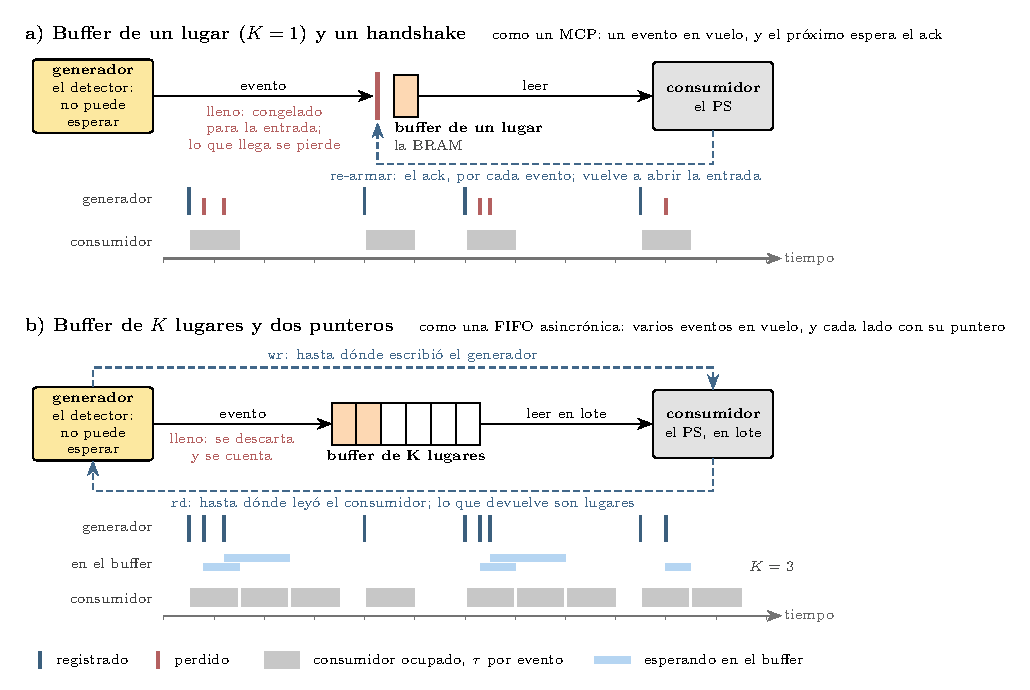
\includegraphics{cap5_productor_consumidor}
\caption[Comunicación inelástica y mediante \emph{pipeline} elástico]{%
Comparación de comunicación inelástica vs comunicación mediante \emph{pipeline}
elástico.\label{f:intro-hw-productor-consumidor}}
\end{figure}

En la Fig.~\ref{f:intro-hw-productor-consumidor}(a) se presenta un
\textbf{sistema no elástico ($K=1$)}: no hay lugar donde esperar, así que la
relación temporal entre productor y consumidor no tiene flexibilidad, y
necesitamos una transacción con la que el consumidor indica que se puede enviar
otro dato. Es lo que llamamos ``armado'', y su mecanismo es exactamente el mismo
del bus \emph{custom}: por eso esta transacción puede interpretarse como un
\codigo{ack}.

En cambio, en el elástico ($K>1$) el generador no tiene que esperar el armado
del consumidor: se desacopla el funcionamiento de cada uno. Ahora cada extremo
depende de una bandera que genera el \emph{buffer}: el generador comprueba que la
bandera \codigo{full} esté baja (todavía queda espacio) y el consumidor observa
la señal \codigo{empty}~\cite{Cummings2002}. Los buses de datos de alto
rendimiento utilizan alguna variación del \emph{pipeline} elástico; por ejemplo, las
interfaces AXI HP contienen FIFOs integradas en la interfaz
PL$\leftrightarrow$PS~\cite{UG585}.

Las tres reglas generales que necesitamos seguir son las siguientes:
\begin{enumerate}
  \item \textbf{Mayor velocidad de procesamiento que de generación}: asegurarse
    de que la metodología de transacciones tenga el \emph{throughput} necesario.
  \item Utilizar \textbf{un \emph{buffer} lo suficientemente grande}: necesitamos un
    criterio de dimensionado, que nos da la teoría de colas
    (Fig.~\ref{f:intro-hw-cola-K}).
  \item \textbf{Saber cuándo fallamos y registrarlo}: tener un mecanismo de
    registro de los tiempos de indisponibilidad o de las fallas.
\end{enumerate}

En nuestros módulos la tasa de generación es la tasa de eventos; en el caso
ideal, la cantidad de partículas detectadas en el experimento. La modifican los
falsos positivos (aumentan los disparos) y los falsos negativos (los reducen).

La tasa de consumo, en cambio, depende del \textbf{tiempo de servicio}: en este
caso, el tiempo que se tarda en pasar un lugar de la FIFO de la PL al PS. Este
largo es fijo y su comienzo depende de cuándo se empieza a ejecutar la
transacción; en el mejor caso el tiempo entre transacciones tiende a cero y
tenemos un consumidor periódico. Podríamos tener varios consumidores trabajando
en paralelo, cada uno con una interfaz AXI dedicada, pero al fin y al cabo,
mientras el \emph{throughput} sea suficiente, el cuello de botella será el dimensionado
del \emph{buffer}.

Este \emph{buffer} se suele denominar circular o anillo (\emph{ring}): no es más que
una cola del tipo FIFO cuyos punteros dan la vuelta al llegar al
final~\cite{Cummings2002}. Si medimos el largo del \emph{buffer} en eventos, es decir,
si la generación y el consumo mueven siempre el mismo largo de datos $B$, el
\emph{buffer} toma valores discretos $K$. Esto aparece en la
Fig.~\ref{f:intro-hw-ring-eventos}: la resta entre los punteros, y no su
posición, dice cuántos lugares quedan libres, y esos lugares son los créditos
del generador.

\begin{figure}[H]
\centering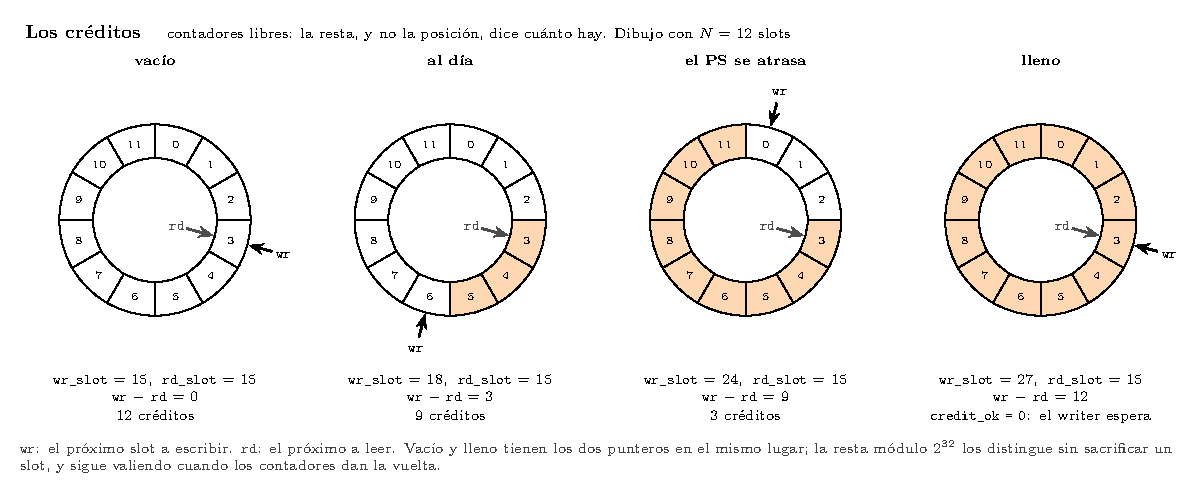
\includegraphics{cap5_ring_creditos}
\caption[Anillo de eventos y cálculo de créditos]{%
Representación de un anillo de eventos y el cálculo de créditos presentes para
cada situación.\label{f:intro-hw-ring-eventos}}
\end{figure}

Cuando no quedan créditos se detiene la sobreescritura fijando el puntero de
escritura \codigo{wr} hasta que el consumidor libere lugar; la cantidad de
ciclos que dura esto es el tiempo de indisponibilidad.

Mientras el \emph{buffer} está congelado, los eventos que llegan se pierden: es tiempo
muerto~\citecap{Knoll2010}{4}. El congelamiento resulta de que tenemos que
mantener fija una región de datos, junto con sus variables de control, hasta que
el consumidor termine de leerla.

De forma que hay dos maneras de reducir el tiempo de indisponibilidad:
\begin{enumerate}
  \item \textbf{Agrandar el \emph{buffer} de datos}: con más lugares de cola, más
    grande es la ráfaga que se puede absorber antes de quedarse sin créditos. La
    Fig.~\ref{f:intro-hw-cola-K} cuantifica cuánto rinde cada lugar.
  \item \textbf{Aumentar el \emph{throughput} de salida}:
  \begin{enumerate}
    \item Procesar varios elementos al mismo tiempo: que cada \emph{slot} se trabaje de
      forma independiente, con su propio conjunto de variables de control. Esto
      es equivalente a tener múltiples punteros de lectura \codigo{rd}, y es el
      acercamiento que empleamos para mejorar el módulo osciloscopio en la
      Sec.~\ref{S:osc-anillo-eventos}.
    \item Leer en lote: el consumidor lee muchos lugares de una vez y los
      devuelve juntos, de modo que el costo fijo de cada transacción se paga una
      vez por lote y no por evento.
  \end{enumerate}
\end{enumerate}

Con un análisis de teoría de colas~\cite{Kendall1953,Gross2008} podemos llegar
a resultados sobre la fracción de eventos perdidos con un productor poissoniano
y un consumidor de tiempo de servicio fijo, que se presentan en la
Fig.~\ref{f:intro-hw-cola-K}. Para $K=1$ no hay cola: si llega un evento con el
consumidor ocupado, se pierde. Con carga baja, $\rho \ll 1$, la pérdida pasa de
$\approx\rho$ a $\approx\rho^K/K!$: cada lugar de cola (aumentar $K$) la baja en
un orden de magnitud o más. Por encima, el consumidor no da abasto en promedio,
ninguna cola alcanza y todas las curvas tienden a $1 - 1/\rho$: el \emph{buffer}
absorbe ráfagas, no un exceso de tasa.

\begin{figure}[H]
\centering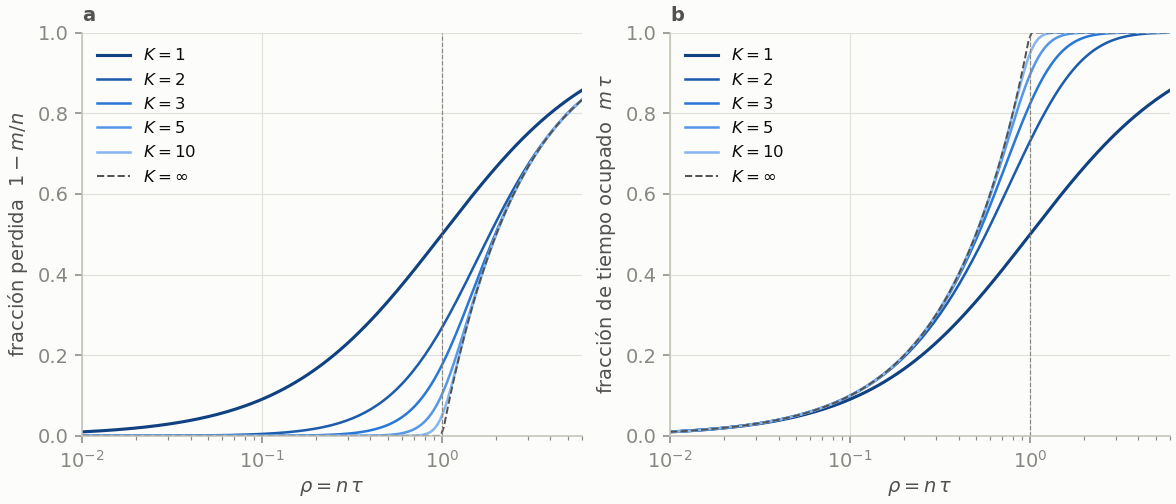
\includegraphics{cap5_cola_K}
\caption[Fracción de eventos perdidos según el largo de cola]{%
(a) Fracción de eventos perdidos en función de la carga $\rho = n\tau$ (tasa
incidente por tiempo de servicio), con arribos Poisson y servicio fijo, para
distintos largos de cola $K$. (b) Fracción del tiempo con el consumidor
ocupado.\label{f:intro-hw-cola-K}}
\end{figure}


\subsubsection{Pérdidas de transacciones por \emph{back-pressure}}
\label{S:intro-hw-back-pressure}

En una red de procesamiento \emph{feed-forward}, es decir, sin ciclos, tenemos
que poner criterios sobre el funcionamiento de los descartes en las ramas
paralelas. En la Fig.~\ref{f:intro-hw-perdida-back-pressure} se presentan los
tres casos típicos. El primero (a) es una cadena estrictamente lineal: los
descartes totales son la suma directa de los descartes de cada etapa. En cambio
(b) y (c) contienen ramas; en (b) las ramas son mutuamente excluyentes, así que
la suma sigue valiendo.

\begin{figure}[H]
\centering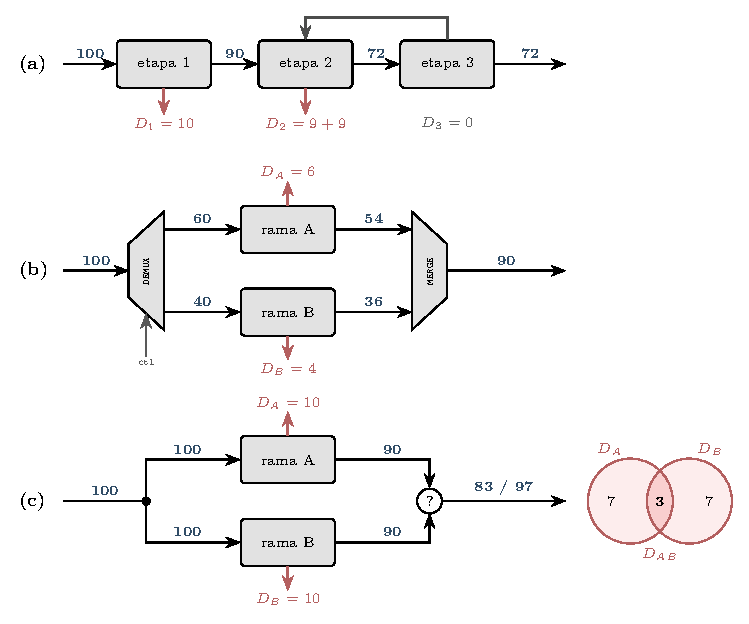
\includegraphics{cap5_perdida_back_pressure}
\caption[Suma de pérdidas en una red \emph{feed-forward}]{%
Cómo se suman las pérdidas en una red de procesamiento \emph{feed-forward}, con
100 eventos de entrada de ejemplo. (a) Cadena lineal: la pérdida total es la
suma de lo que descarta cada etapa. (b) Ramas exclusivas: ningún evento está en
las dos ramas y la suma sigue valiendo. (c) Ramas no exclusivas: la pérdida
depende de qué cuenta como sobrevivir, y la suma de los contadores cuenta dos
veces los eventos perdidos en las dos
ramas.\label{f:intro-hw-perdida-back-pressure}}
\end{figure}

El dilema aparece con dos ramas que no son mutuamente excluyentes (c), porque el
criterio de descarte sale de la lógica local de cada bloque. En este ejemplo
podríamos tener como criterio que un evento se pierda sólo si ambas ramas fallan
simultáneamente, y entonces la suma de los 10 descartes que reporta cada bloque
no refleja el valor final. Una forma de arreglarlo es diseñar la red de forma
que los elementos de las ramas paralelas no puedan descartar, sino sólo
bloquear la entrada hasta la etapa anterior al punto donde se separan las ramas,
y contar los descartes en la sección secuencial. Esto significa que no todos los
bloques descartan: algunos \textbf{bloquean} el flujo de datos, y ese bloqueo que
se propaga hacia atrás es la \emph{back-pressure}
(contrapresión)~\cite[caps.~12 y 13]{Dally2004}.

Que un bloque descarte o bloquee depende del esquema de comunicación de cada
etapa. Por ejemplo, un ADC trabaja en modo \emph{fire and forget}: su salida no
tiene control de flujo ni confirmación de llegada, mientras que los elementos
dentro de la cadena sí los tienen. La consecuencia a nivel de bloque es que
donde la comunicación es unidireccional, es decir, donde \textbf{no vemos flecha
de vuelta}, el sistema puede descartar.

Esto quiere decir que los bloques no necesariamente avanzan en todos los ciclos
de reloj: como los eventos llegan a una tasa mucho menor que la del reloj, la
cadena no necesita procesar uno por ciclo, y eso nos deja implementar mecanismos
de control más complejos.

Lo que importa es cómo se traduce el bloqueo en descartes
(Fig.~\ref{f:intro-hw-etapas-descartes}): si la \emph{back-pressure} llega hasta
un bloque con una entrada ininterrumpida, como un ADC, tenemos un descarte.

\begin{figure}[H]
\centering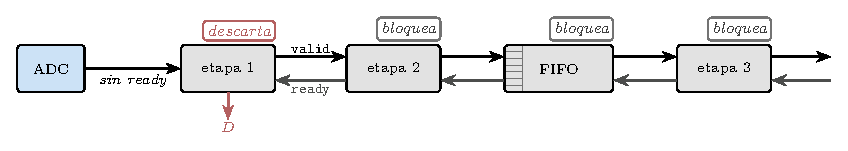
\includegraphics{cap5_etapas_vs_descartes}
\caption[Descartes y bloqueos de las etapas de procesamiento]{%
Descartes y bloqueos de las etapas de
procesamiento.\label{f:intro-hw-etapas-descartes}}
\end{figure}

%==============================================================================
\section{Bus \emph{custom} de RedPitaya}
\label{S:intro-hw-bus-custom}

El bus \emph{custom} de Red Pitaya~\cite{RedPitayaFPGA} puede emplear cualquiera de los
mecanismos de transferencia explicados en la Sec.~\ref{S:intro-hw-transferencia}
en los que la PL funciona como \emph{slave}. Cada operación sobre este bus representa
una flecha de la Fig.~\ref{f:intro-hw-tipos-control}. En todos los módulos que
usan este bus utilizamos el esquema de \emph{handshake} completo.

Los elementos conectados a él tienen que implementar la decodificación de
direcciones y respetar un ordenamiento en el acceso: como hay un único
\codigo{ack}, todos los módulos deben \textbf{turnarse la utilización del bus}.
En la Fig.~\ref{f:intro-hw-fsm-bus} se presenta la máquina de estados que
\textbf{sigue el bus} \emph{custom} de Red Pitaya. A esta secuencia de pasos se la suele
denominar \textbf{contrato}, porque la FSM no se implementa explícitamente: se
diseñan \emph{slaves} y \emph{masters} que cumplen sólo lo que se le exige a cada extremo.
Esto se refleja en optimizaciones, simplificaciones y consideraciones
importantes para su diseño y uso. Los pasos son:
\begin{enumerate}
  \item \textbf{Reposo}: el bus está libre, con \codigo{wen} y \codigo{ren}
    en~0.
  \item \textbf{Pedido}: el maestro pone \codigo{addr} (y \codigo{wdata}, si es
    escritura) y levanta \codigo{wen} o \codigo{ren}. El esclavo ejecuta la
    escritura, o lanza la lectura, una sola vez, con un estrobo de un ciclo.
  \item \textbf{Espera}: \codigo{wen}/\codigo{ren} siguen en alto y
    \codigo{addr} y \codigo{wdata} quedan quietos hasta el \codigo{ack}. Del
    lado del esclavo no hay \emph{timeout}: si el \codigo{ack} no llega, el \emph{slot} se
    queda en este estado. El maestro sí tiene uno, que se describe en la
    Sec.~\ref{S:intro-hw-modos-falla}.
  \item \textbf{\emph{Acknowledge}}: el esclavo levanta \codigo{ack}, con
    \codigo{rdata} ya registrado en el caso de una lectura. El maestro lo ve,
    baja \codigo{wen}/\codigo{ren}, y el bus vuelve a reposo.
\end{enumerate}

\begin{figure}[H]
\centering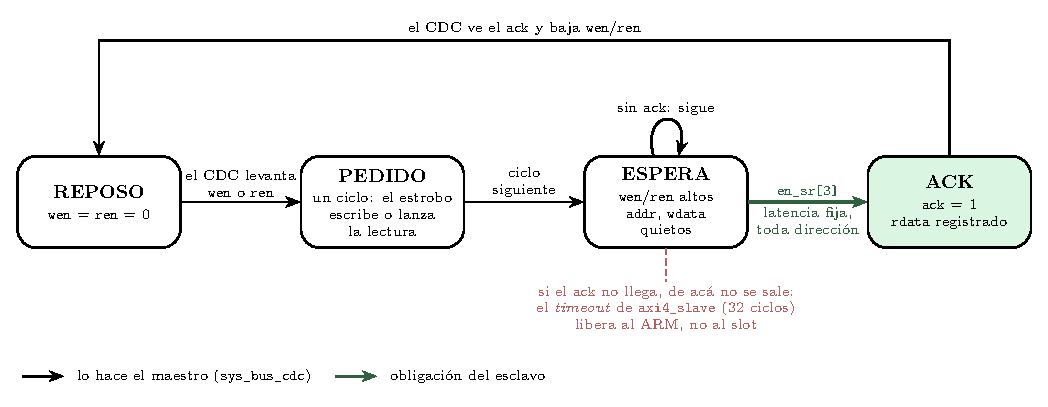
\includegraphics{cap5_contrato_sys_bus}
\caption[Contrato del bus \emph{custom} de Red Pitaya]{%
Diagrama del bus \emph{custom} de RedPitaya. Contiene cuatro
estados.\label{f:intro-hw-fsm-bus}}
\end{figure}

La única obligación del esclavo es la del paso~4: responder a toda dirección de
su \emph{slot} (que la \emph{request} sea para él), mapeada o no, con latencia fija.

\subsection{Rendimiento del bus}
\label{S:intro-hw-rendimiento-bus}

La Fig.~\ref{f:intro-hw-camino-bus} presenta las 4 etapas de una lectura o
escritura de 32 bits por el bus \emph{custom} de Red Pitaya a un \emph{slave} genérico.

\begin{figure}[H]
\centering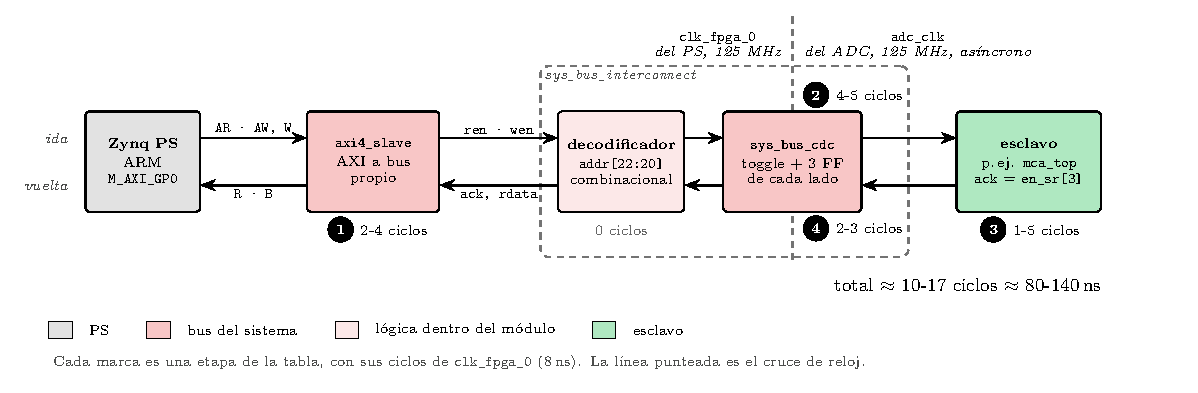
\includegraphics{cap5_latencia_sys_bus}
\caption[Camino de una transferencia por el bus \emph{custom}]{%
Flujo de comunicación para una transferencia PS$\rightarrow$\emph{slave} de la PL
mediante el bus \emph{custom}.\label{f:intro-hw-camino-bus}}
\end{figure}

Arrancamos con el camino PS$\rightarrow$PL, que pasa por el
\codigo{axi4\_slave} con una latencia de 2 a 4 ciclos según la transacción: 2
para la lectura y hasta 4 para la escritura, según el orden de llegada de la
dirección y los datos. Los cruces \codigo{clk\_fpga0} $\rightarrow$
\codigo{adc\_clk} (paso~2) y \codigo{adc\_clk} $\rightarrow$
\codigo{clk\_fpga0} (paso~4) usan el mismo CDC, un \emph{handshake} por
\emph{toggle}~\cite{Cummings2008} de 4 a 5 ciclos. La variación se debe a que depende
de la diferencia de fase entre los relojes.

En la Tabla~\ref{t:intro-hw-rendimiento-bus} se describe cada uno de estos pasos
y se calcula la latencia total de la comunicación. Los valores de cada etapa son
los del diseño de Red Pitaya, y los del CDC no conviene achicarlos: para relojes
asincrónicos, sin relación de frecuencia fraccional, la tasa de fallas por
metaestabilidad crece de forma exponencial al reducir el tiempo de
sincronización~\cite{Ginosar2011}. Para el esclavo se consideró uno genérico,
con un tiempo de respuesta de hasta 5 ciclos.

Cuando ambos dominios tienen la misma frecuencia, las sincronizaciones de ida y
de vuelta suelen ser instancias de un mismo módulo, y por eso los ciclos
requeridos en ambos trayectos son iguales. Cuando la relación de frecuencias es
mayor, $f_\text{max} > 2f_\text{min}$, podríamos utilizar otros esquemas de
sincronización, en los que se diferencian los caminos \emph{fast-to-slow} y
\emph{slow-to-fast}~\cite{Cummings2008}.

\begin{table}[H]
\centering
\caption[Latencia de una transacción del bus \emph{custom}]{%
Estimados de latencia por etapa y total para una transacción del bus \emph{custom} de
RedPitaya.\label{t:intro-hw-rendimiento-bus}}
\begin{tabular}{|c|l|l|}
\hline \encabezado \textbf{\#} & \textbf{Etapa} & \textbf{Ciclos requeridos}
  \\ \hline
1 & AXI + \codigo{axi4\_slave} & 2--4 \\ \hline
2 & CDC ida (\emph{toggle} + 2--3 \emph{flops}) & 4--5 \\ \hline
3 & Esclavo & 1--5 \\ \hline
4 & CDC vuelta & 4--5 \\ \hline
  & \textbf{Total} & \textbf{$\sim$12--20} $\approx$
    \qtyrange{100}{160}{\nano\second} \\ \hline
\end{tabular}
\end{table}

Estas latencias provienen de que los dos extremos no comparten reloj. Es una
cuestión de \emph{trade-off}: no vale la pena quitar el problema de raíz si sincronizar
los relojes es tan costoso en HW y podemos diseñar sistemas que compensen
parcialmente sus efectos, como el \emph{pipeline} elástico.

\subsection{\emph{Waveforms} de transacciones por \texttt{axi4\_slave}}
\label{S:intro-hw-waveforms-axi}

En la Fig.~\ref{f:intro-hw-escritura} presentamos una \emph{waveform} de una
transferencia de escritura del parámetro \codigo{cfg\_amp\_max} (de dirección
\codigo{0x4070\_0034}) obtenida por simulación. Se tienen los siguientes pasos:
\begin{enumerate}
  \item \emph{Master}: pone los valores de \codigo{addr} y \codigo{wdata} y levanta
    \codigo{wen} (ciclo~2).
  \item \emph{Slave}: ve el cambio en \codigo{wen} (\qty{35}{\nano\second} después) y
    genera una operación de un ciclo (\textbf{estrobo}); en el flanco siguiente
    \codigo{cfg\_amp\_max} toma el valor de \codigo{wdata} (ciclo~8).
  \item \emph{Slave}: con la latencia fija del módulo, sube \codigo{sys\_ack}
    (ciclo~12).
  \item \emph{Master}: ve el \codigo{ack} ya sincronizado (\qty{96}{\nano\second}
    después de iniciar la transacción) y baja \codigo{wen}, completando la
    transacción.
\end{enumerate}

En la lectura se mantienen los roles \emph{master}/\emph{slave} y la transacción es casi
idéntica; se puede ver en la Fig.~\ref{f:intro-hw-lectura}. Sus diferencias son
las siguientes:
\begin{enumerate}
  \item \emph{Master}: fija únicamente \codigo{addr} (no pone \codigo{wdata}) y
    levanta \codigo{ren} en vez de \codigo{wen} (ciclo~2).
  \item \emph{Slave}: el valor de \codigo{rdata} hay que tomarlo cuando \codigo{ack}
    está en alto (ciclo~17).
\end{enumerate}

% Las dos waveforms son muy anchas (20 x 5 pulgadas): van juntas en una página
% apaisada, cada una con su número y epígrafe.
\begin{figuraapaisada}
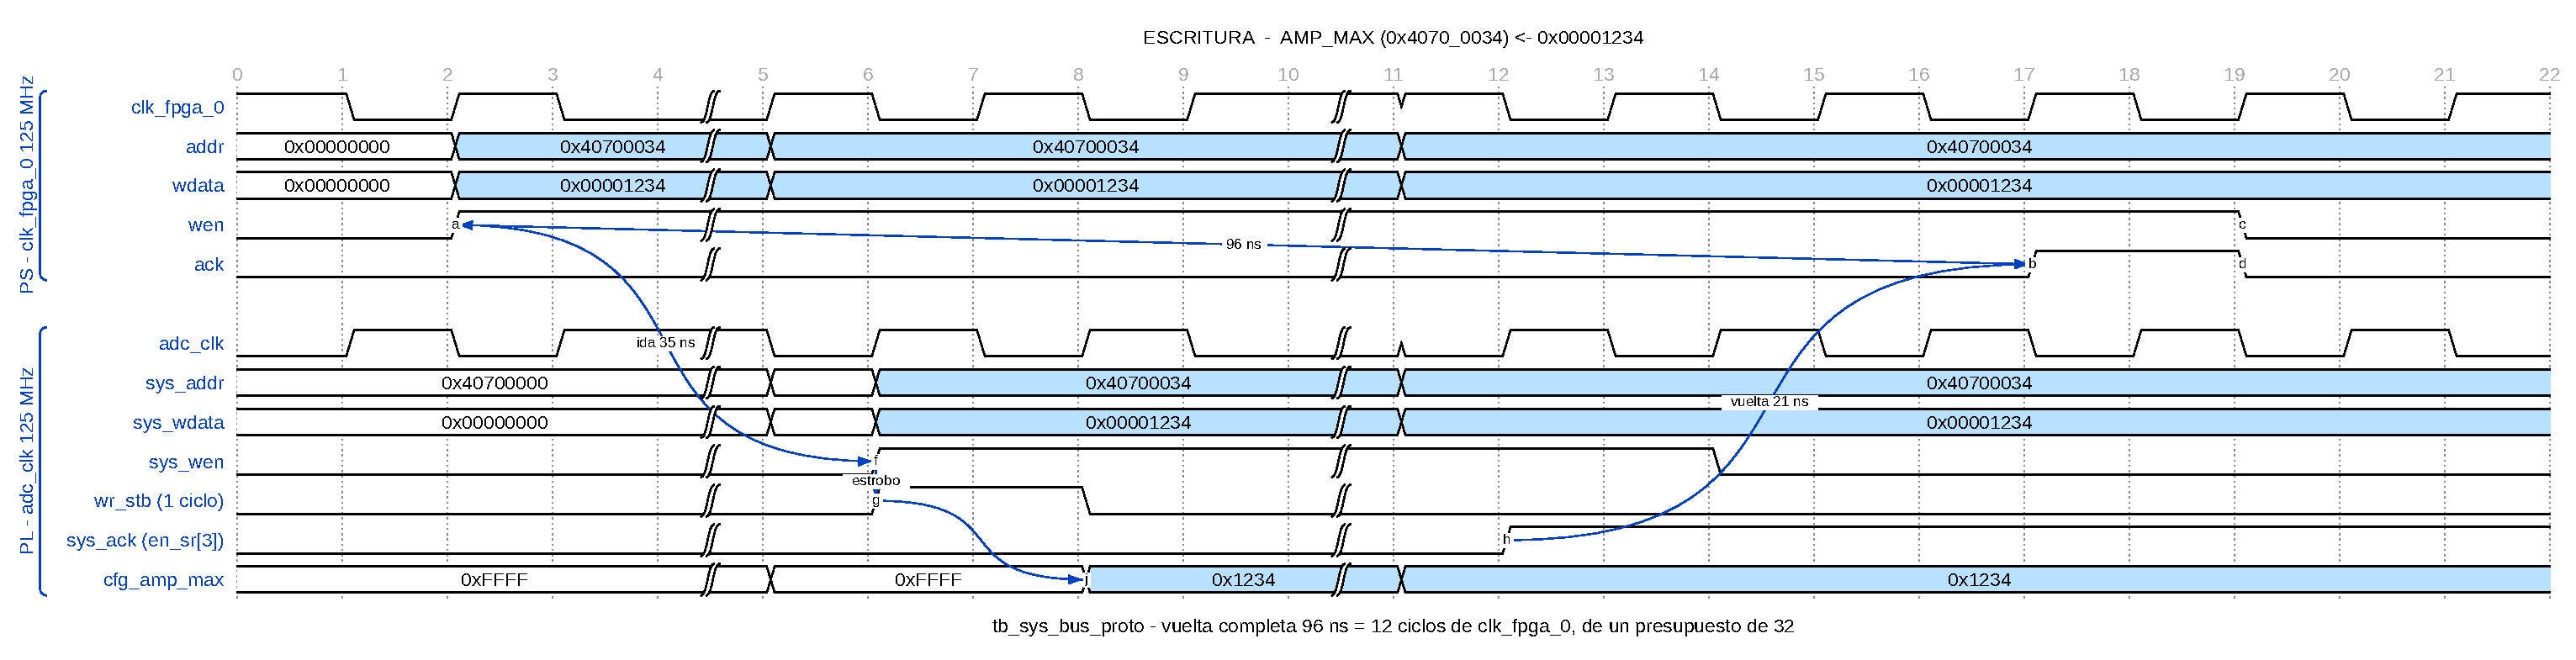
\includegraphics[height=0.4\textwidth]{cap5_bus_escritura}
\caption[\emph{Waveform} simulada de una escritura por el bus \emph{custom}]{%
\emph{Waveform} simulada de la transacción de escritura al registro
\codigo{AMP\_MAX}, de dirección \codigo{0x4070\_0034}, con el valor
\codigo{0x1234}.\label{f:intro-hw-escritura}}

\vspace{2\baselineskip}
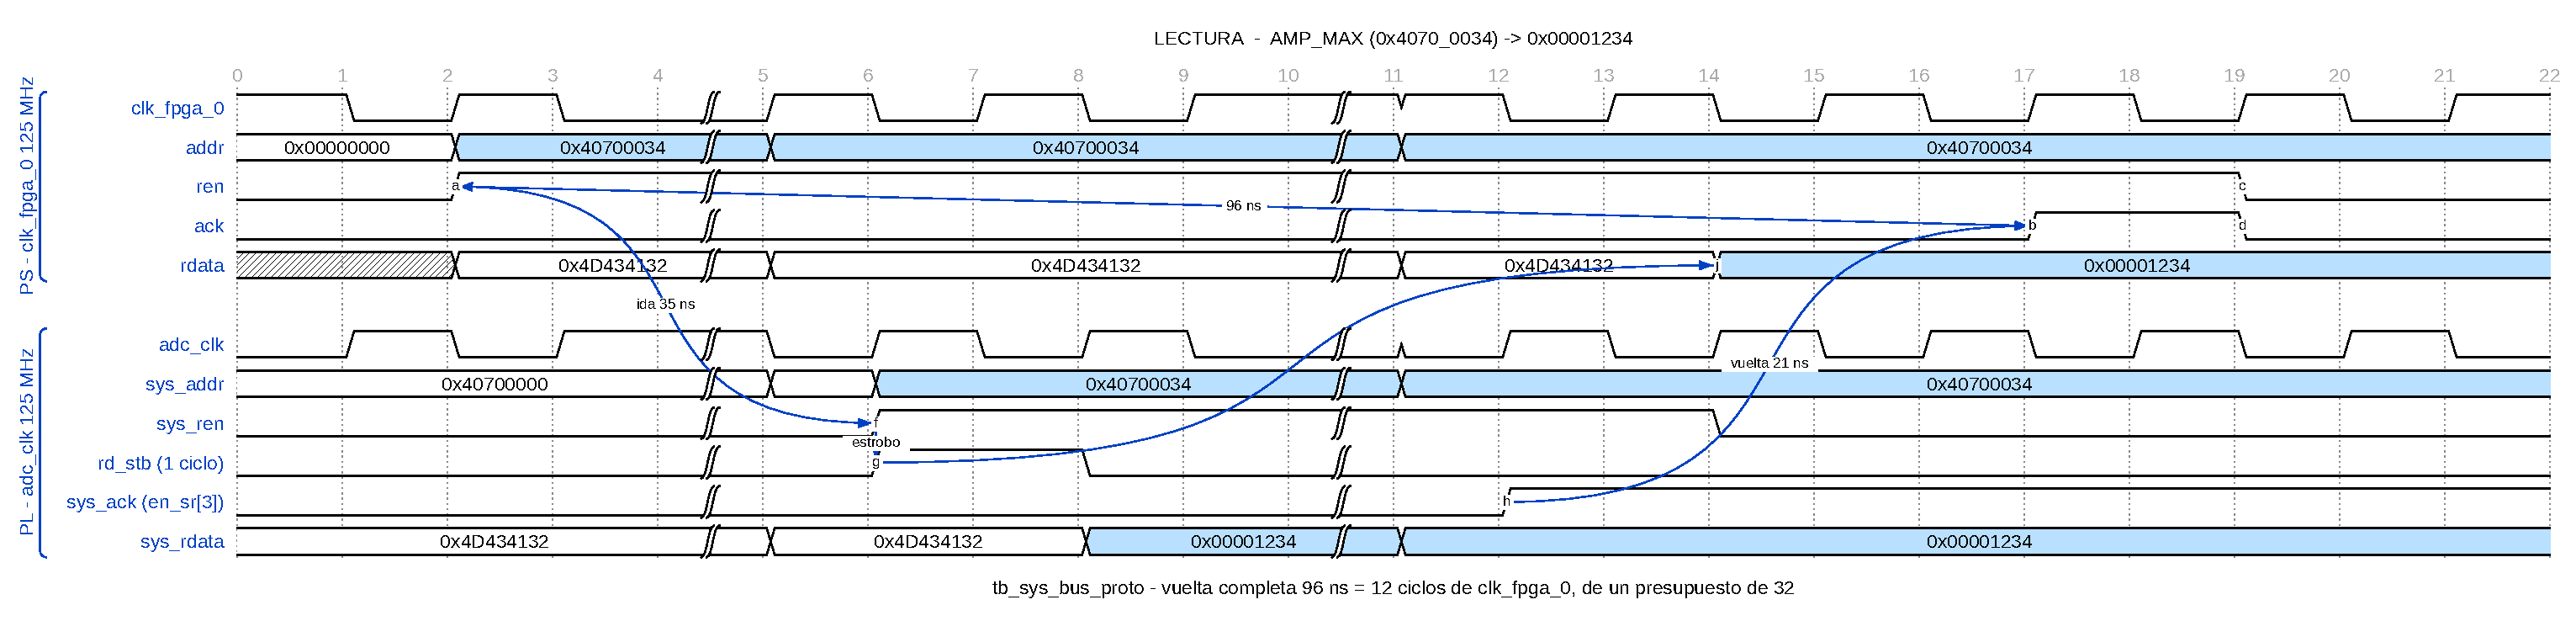
\includegraphics[height=0.4\textwidth]{cap5_bus_lectura}
\caption[\emph{Waveform} simulada de una lectura por el bus \emph{custom}]{%
\emph{Waveform} simulada de la transacción de lectura al registro \codigo{AMP\_MAX},
de dirección \codigo{0x4070\_0034}.\label{f:intro-hw-lectura}}
\end{figuraapaisada}

\subsection{Mapa de registros}
\label{S:intro-hw-mapa-registros}

Es una tabla en la que asociamos \textbf{direcciones físicas y permisos de
acceso} a los registros de control y de estado de un módulo. Los módulos
empleados tienen dos clases de parámetros: los compartidos y los específicos de
cada \emph{stream} de datos. Lo que suele hacerse es colocar las configuraciones
compartidas en la base de la estructura y después la configuración de cada uno
de los bloques, de forma individual.

Cada módulo tiene \textbf{su mapa de registros local}, que en la etapa de
integración se ubica en el mapa de memoria del sistema mediante un \emph{offset} fijo.
Esto simplifica el SW, porque entre las configuraciones de los bloques hay un
salto fijo, llamado \textbf{\emph{stride}}: las estructuras quedan compactas y se
representan fácilmente con \emph{structs} de C.

En la Fig.~\ref{f:intro-hw-mapa-registros} se presenta, de izquierda a derecha,
el mapa de direcciones físicas de la PL, que tiene que coincidir con el que ve el
PS~\cite{UG585}. Consta de 8 regiones de 1~MB cada una. El segundo \emph{slot} es el
mapa de direcciones del módulo osciloscopio, que repite las direcciones previas
(el mapa \emph{legacy}) para que la API precompilada de Red Pitaya siga siendo
compatible.

\begin{figure}[H]
\centering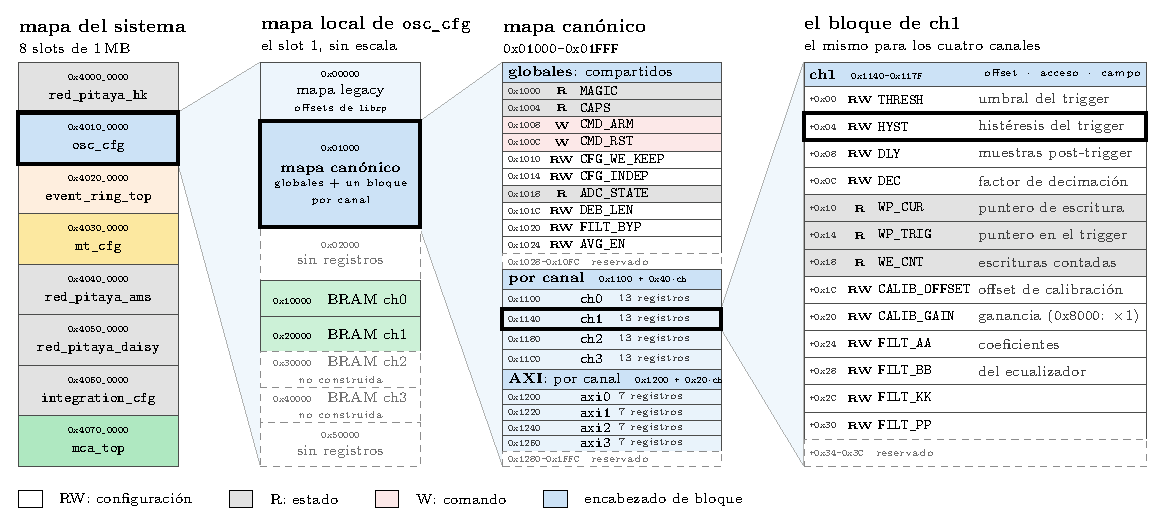
\includegraphics{cap5_mapa_registros_osc}
\caption[Cuatro escalas del mapa de registros]{%
Cuatro escalas del mapa de registros. (a) Nivel sistema. (b) Nivel módulo:
contiene datos (ver BRAM presente). (c) Nivel configuración de módulo. (d) Nivel
configuración de un canal.\label{f:intro-hw-mapa-registros}}
\end{figure}

Al realizar una transacción, el sistema analiza los prefijos de la dirección
para averiguar cómo rutear la transferencia: por ejemplo, como la dirección
arranca con \codigo{b0100000}, el PS sabe de entrada que le corresponde la
interfaz AXI GP0~\cite{UG585}. Después la dirección la lee el
\codigo{sys\_bus\_interconnect}, que decodifica el \emph{slot} dentro del mapa de
memoria global y redirige la transacción al módulo de sincronización asociado.
En la Fig.~\ref{f:intro-hw-calculo-direccion} se pueden ver las distintas capas
de direccionamiento para la dirección \codigo{0x4010\_1144}, que pertenece al
registro \codigo{HYST} del canal~1 del \emph{slot}~1 (OSC).

\begin{figure}[H]
\centering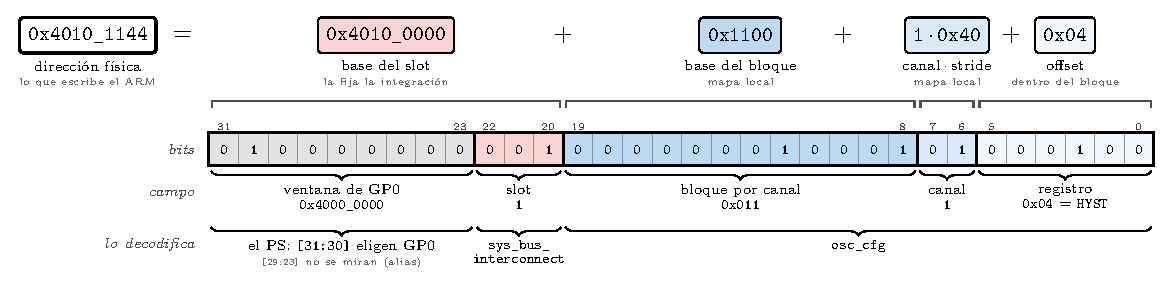
\includegraphics{cap5_calculo_direccion_osc}
\caption[Enrutamiento de una dirección según regiones de memoria]{%
Ejemplo de enrutamiento según regiones de
memoria.\label{f:intro-hw-calculo-direccion}}
\end{figure}

Es interesante notar que la dirección queda asociada a la interfaz GP0. Si la PL
tuviera el mismo \emph{slave} conectado también a la otra interfaz maestra del PS, la
GP1, podríamos asociar \textbf{el mismo registro a otra región de memoria} y
acceder a él por ese otro camino de datos. Las interfaces HP no sirven para
esto: en ellas el \emph{master} es la PL.

\subsection{Modos de falla del bus interno}
\label{S:intro-hw-modos-falla}

A continuación comentamos las formas de llevar el sistema a un estado erróneo.
Son fallas que exceden al módulo que las provoca: aparecen en la interacción
entre el PS, el \codigo{axi4\_slave} y el \emph{slave}.
\begin{enumerate}
  \item \textbf{\emph{Slave} que no hace \codigo{ack}}: los \emph{slaves} comparten el recurso
    que representa el bus. Si un \emph{slave} no hace \codigo{ack}, su \emph{slot} queda en el
    estado de espera de la Fig.~\ref{f:intro-hw-fsm-bus} y el CDC de ese \emph{slot}
    queda desincronizado: es un \textbf{\emph{deadlock}} latente del \emph{slot}, y las
    transacciones siguientes a ese \emph{slot} salen corruptas. El PS no se cuelga
    porque el \codigo{axi4\_slave} tiene un \emph{timeout}: a los 32 ciclos
    fabrica el \codigo{ack} y responde con error
    (\codigo{SLVERR})~\cite{AMBAAXI,RedPitayaFPGA}, que el ARM recibe como un
    \emph{external abort}. Por eso un \emph{slave} tiene que hacer \codigo{ack} de toda
    dirección de su \emph{slot}, mapeada o no; el \emph{timeout} es una red de seguridad, no
    parte del contrato.
  \item \textbf{Ráfagas y anchos incorrectos}: el \codigo{axi4\_slave} que
    conecta el bus \emph{custom} implementa una versión reducida de AXI: no acepta
    transferencias en ráfaga ni accesos anchos, sólo \codigo{LEN = 0} y
    \codigo{SIZE} de 2 o 4 bytes~\cite{AMBAAXI}. Cualquier otra transacción la
    rechaza con \codigo{SLVERR} sin que llegue al \emph{slave}. Esto es importante
    porque limita las instrucciones que podemos usar desde el PS; se expande
    este tema en la Sec.~\ref{S:sw-modos-fallo}.
\end{enumerate}

Es un buen ejemplo de por qué conviene conocer el modelo de memoria del
procesador~\cite{DDI0406C}: el \emph{bug} no está ni en el RTL ni en el código Python,
sino en la interacción entre lo que la ISA permite emitir y lo que el esclavo
acepta recibir.

\subsection{Módulo de configuración}
\label{S:intro-hw-modulo-config}

Los módulos implementados tienen un submódulo de configuración, por ejemplo
\codigo{mt\_cfg}, \codigo{osc\_cfg} e \codigo{integration\_cfg}; en el MCA la
misma lógica está dentro de \codigo{mca\_top}. Es el que \textbf{implementa el
acceso por un mapa de registros} y la transferencia al bus \textbf{\emph{custom}}.
Todos repiten la misma estructura; en la Fig.~\ref{f:intro-hw-panorama-cfg} se
presenta una versión tipo plantilla. Los bloques en gris son plantillas que
contienen los elementos \emph{ad hoc} que requiera el diseño:
\begin{itemize}
  \item \textbf{Comandos}: generalmente generan señales de un ciclo de reloj que
    arrancan un comando, representado por una FSM en el módulo.
  \item \textbf{Registros de configuración}: generalmente son señales lentas.
  \item \textbf{Identificación}: un número fijo en el HW con el que se puede
    diagnosticar rápidamente si la carga del \emph{bitstream} en la placa fue exitosa;
    se lo utiliza para identificar el módulo y comprobar la versión.
  \item \textbf{Lógica}: el resto de los elementos que no entran en las
    categorías previas, por ejemplo los registros tipo \emph{snapshot}.
\end{itemize}
Los bloques en rojo claro representan bloques de RTL fijos para todos los
módulos de configuración:
\begin{itemize}
  \item \textbf{Escritura}: un decodificador de dirección traduce el \emph{offset}
    (\codigo{sys\_addr[19:0]}) en la habilitación del registro que le
    corresponde, y ese registro copia su campo de \codigo{sys\_wdata}.
  \item \textbf{Estrobo}: \codigo{sys\_wen} queda alto hasta el \codigo{ack},
    unos 5 ciclos. El estrobo lo convierte en un pulso de un ciclo
    (\codigo{wr\_stb = sys\_wen \&\& !en\_sr[0]}), para que cada
    \textbf{escritura se ejecute una sola vez}.
  \item \textbf{\emph{Ack}}: sale de un registro de desplazamiento sobre
    \codigo{sys\_en = sys\_wen | sys\_ren}, con latencia fija y para cualquier
    dirección, mapeada o no. \codigo{sys\_err} vale siempre~0.
  \item \textbf{Lectura}: un multiplexor controlado por la misma dirección elige
    qué va a \codigo{sys\_rdata}. Puede ser el valor escrito, el estado y los
    contadores de la región, la identificación o, en los módulos con memoria,
    una ventana de BRAM o de histograma. Las direcciones no mapeadas leen~0. La
    salida del multiplexor pasa por un registro: \codigo{sys\_rdata} cruza al
    dominio de reloj del PS sin sincronizador~\cite{Cummings2008} y con menos de
    \qty{1}{\nano\second} de margen, así que no puede llevar lógica
    combinacional.
\end{itemize}

\begin{figure}[H]
\centering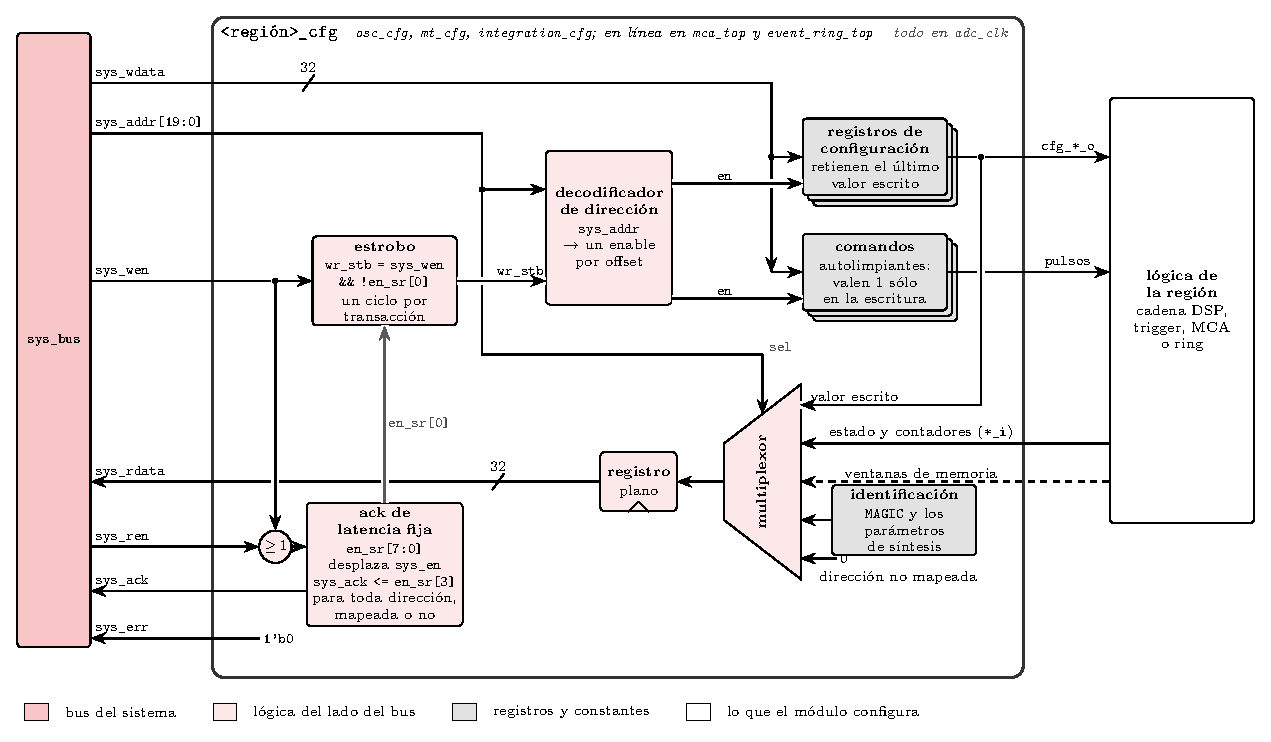
\includegraphics{cap5_panorama_modulo_cfg}
\caption[Plantilla del módulo de configuración]{%
\emph{Template} del módulo de configuración, incluye conexión al bus \emph{custom} de
RedPitaya.\label{f:intro-hw-panorama-cfg}}
\end{figure}

Ahora que terminamos de ver los temas generales del diseño de HW, tenemos que
ver cómo comprobamos su funcionamiento: este es el dominio de la verificación.

%==============================================================================
\section{Verificación}
\label{S:intro-hw-verificacion}

Quien haya trabajado en diseño de HW sabe lo exhaustiva que puede volverse la
verificación previa a la síntesis: se lleva una fracción importante del tiempo
de los proyectos de FPGA~\cite{Foster2022}. A nuestro entender, se debe
principalmente a los siguientes elementos:
\begin{itemize}
  \item No tenemos herramientas de \emph{debug} intrínsecas al hardware realizado:
  \begin{itemize}
    \item A diferencia del SW, en el que tenemos un \emph{debugger} para diagnosticar
      los errores en tiempo de ejecución, en HW no tenemos estas capacidades a
      menos que exportemos las señales hacia afuera, por ejemplo con un
      analizador lógico integrado en la FPGA, que consume recursos y sólo ve las
      señales que elegimos antes de sintetizar.
  \end{itemize}
  \item El \textbf{espacio de entradas} de un módulo puede ser
    \textbf{arbitrariamente grande}, y su espacio de estados crece de forma
    exponencial con la cantidad de registros.
  \begin{itemize}
    \item En cada ciclo todas las entradas tienen un valor, así que hay que
      analizar el efecto de todas las entradas del módulo en todos los ciclos.
    \item Acordémonos de que el punto más fuerte de estas plataformas es el
      paralelismo: muchas cosas pasan en el mismo ciclo, y las combinaciones de
      eventos simultáneos se multiplican.
  \end{itemize}
  \item Trabajamos en escalas temporales muy distintas:
  \begin{itemize}
    \item Como ejemplo, nuestra placa trabaja a \qty{125}{\mega\hertz}: un
      segundo de funcionamiento son $1,25\cdot10^{8}$ ciclos. Una falla que
      aparece una vez cada millón de ciclos se ve en la placa en milisegundos,
      pero en simulación exige corridas larguísimas o un estímulo dirigido que
      la provoque.
  \end{itemize}
\end{itemize}

\subsection{Técnicas de verificación}
\label{S:intro-hw-tecnicas}

Tenemos una variedad de técnicas y herramientas para verificar tanto la
funcionalidad como la factibilidad; en la Tabla~\ref{t:intro-hw-tecnicas}
aparece qué detecta cada una.

\begin{table}[H]
\centering
\caption[Qué detecta cada técnica de verificación]{%
Qué detecta cada una de las técnicas de verificación más empleadas.
$^{*}$Sólo para las propiedades que se escriban.\label{t:intro-hw-tecnicas}}
\begin{tabularx}{\textwidth}{|X|c|c|c|c|}
\hline \encabezado & \textbf{Lint} & \textbf{STA} &
  \textbf{\emph{Golden model} + \emph{coverage}} & \textbf{Formal} \\ \hline
Error de sintaxis & sí & no & sí & sí \\ \hline
\emph{Latch} inferido & \textbf{sí} & no & parcial & no \\ \hline
Ancho que no coincide & \textbf{sí} & no & parcial & no \\ \hline
\emph{Bug} funcional & no & no & \textbf{sí} & sí$^{*}$ \\ \hline
Camino crítico & no & \textbf{sí} & no & no \\ \hline
Cruce de dominios de reloj (CDC) & parcial & \textbf{no} & no & parcial
  \\ \hline
Equivalencia RTL/netlist & no & no & parcial & \textbf{sí} \\ \hline
\textbf{Importancia} & Media & Crítica & Alta & Baja \\ \hline
\end{tabularx}
\end{table}

Los puntos fuertes de cada técnica son:
\begin{itemize}
  \item El \textbf{lint} consiste en un \textbf{análisis estático} del código de
    descripción de hardware para asegurar que cumple ciertas reglas,
    generalmente las ``buenas prácticas'' de la industria~\cite{Keating2002}.
    Reporta advertencias sobre las inferencias del sintetizador que suelen ser
    problemáticas, porque su depuración puede ser muy compleja: anchos que no
    coinciden e inferencias no deseadas, usualmente \emph{latches}. Los problemas de
    \emph{clock domain crossing} (CDC) se revisan con un análisis estructural
    del mismo tipo pero dedicado, que busca las señales que cruzan de dominio
    sin sincronizador~\cite{Cummings2008}.
  \item El \textbf{STA} (\emph{static timing analysis}) asegura que el sistema
    \textbf{funcione a nivel temporal}, es decir, que valga la abstracción
    sincrónica: que toda señal llegue a su registro dentro del período de
    reloj~\cite{Bhasker2009}. Los caminos entre relojes asincrónicos se
    declaran como excepciones y no se analizan; por eso no detecta problemas de
    CDC.
  \item El \textbf{\emph{golden model}} (``modelo dorado'') es un modelo de referencia,
    escrito aparte y en un lenguaje de más alto nivel, contra el que se compara
    la salida del RTL; nos asegura que el módulo \textbf{funciona a nivel de
    transacciones}~\cite{Bergeron2003}. El \emph{coverage} nos da una noción de
    cuánto del código o del espacio de señales se probó realmente.
  \item La verificación \textbf{formal} es una \textbf{demostración
    exhaustiva}, mediante métodos matemáticos, de que el sistema no puede
    llegar a estados inválidos~\cite{Seligman2023}. Se aplica normalmente para
    asegurar que no se presente un \textbf{\emph{deadlock}}, y en su variante de
    equivalencia compara el RTL contra la netlist sintetizada.
\end{itemize}

\subsection{Exploración del espacio de entrada}
\label{S:intro-hw-formal}

Este análisis se realiza de forma exhaustiva mediante motores de demostración
que prueban propiedades, y se llama comúnmente \textbf{análisis
formal}~\cite{Seligman2023}. Se quieren dar las siguientes dos garantías:
\begin{enumerate}
  \item El sistema no llega a estados inválidos:
  \begin{enumerate}
    \item Se parte de la secuencia de \emph{reset} y se recorren todas las secuencias
      de entrada válidas hasta una profundidad de $k$ ciclos (\emph{bounded
      model checking})~\cite{Biere1999}.
    \item Se demuestra que, desde cualquier estado válido y con una entrada
      válida, el sistema permanece en un estado válido. Junto con el punto
      anterior es una demostración por inducción, que vale para cualquier
      cantidad de ciclos~\cite{Sheeran2000}.
  \end{enumerate}
  \item No se emiten transacciones inválidas durante la ejecución:
  \begin{enumerate}
    \item Se respeta la secuencia de cada transacción. Por ejemplo, si tuvimos
      dos \emph{requests} tenemos que tener dos \emph{responses}, y ninguna
      \emph{response} sin su \emph{request}.
    \item Los datos siguen nuestro modelo propuesto: lo que sale del módulo
      coincide con lo que predice el \emph{golden model} para las mismas entradas.
  \end{enumerate}
\end{enumerate}

% Bibliografía de este capítulo. Va al final del archivo, siempre.
\bibliografiacapitulo

%%% Local Variables:
%%% mode: latex
%%% TeX-master: "template"
%%% End:
